\documentclass[14pt]{extbook}
\usepackage{multicol, enumerate, enumitem, hyperref, color, soul, setspace, parskip, fancyhdr} %General Packages
\usepackage{amssymb, amsthm, amsmath, bbm, latexsym, units, mathtools} %Math Packages
\everymath{\displaystyle} %All math in Display Style
% Packages with additional options
\usepackage[headsep=0.5cm,headheight=12pt, left=1 in,right= 1 in,top= 1 in,bottom= 1 in]{geometry}
\usepackage[usenames,dvipsnames]{xcolor}
\usepackage{dashrule}  % Package to use the command below to create lines between items
\newcommand{\litem}[1]{\item#1\hspace*{-1cm}\rule{\textwidth}{0.4pt}}
\pagestyle{fancy}
\lhead{Progress Quiz 4}
\chead{}
\rhead{Version A}
\lfoot{4378-7085}
\cfoot{}
\rfoot{Fall 2020}
\begin{document}

\begin{enumerate}
\litem{
Choose the graph of the equation below.\[ f(x) = \frac{-1}{(x + 1)^2} - 3 \]\begin{enumerate}[label=\Alph*.]
\begin{multicols}{2}\item 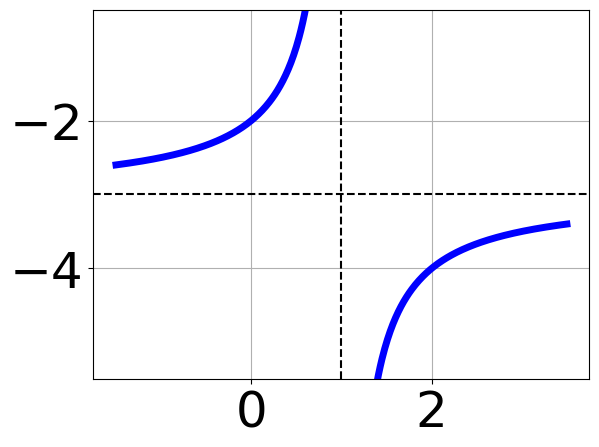
\includegraphics[width = 0.3\textwidth]{../Figures/rationalEquationToGraphCopyAA.png}\item 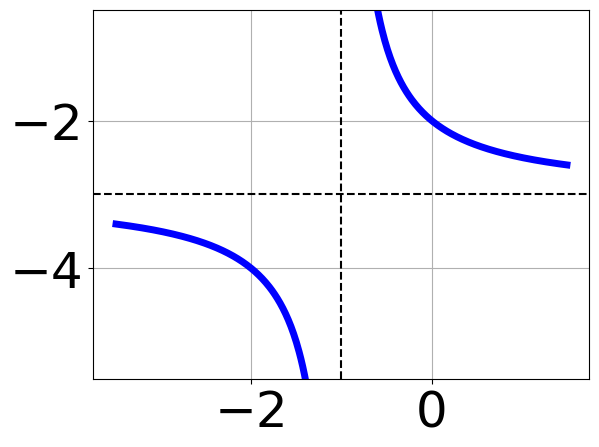
\includegraphics[width = 0.3\textwidth]{../Figures/rationalEquationToGraphCopyBA.png}\item 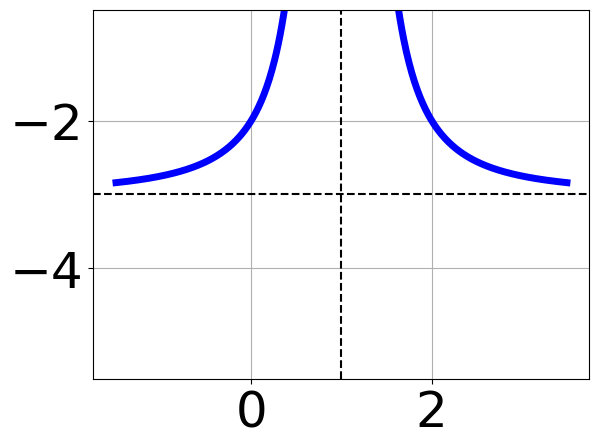
\includegraphics[width = 0.3\textwidth]{../Figures/rationalEquationToGraphCopyCA.png}\item 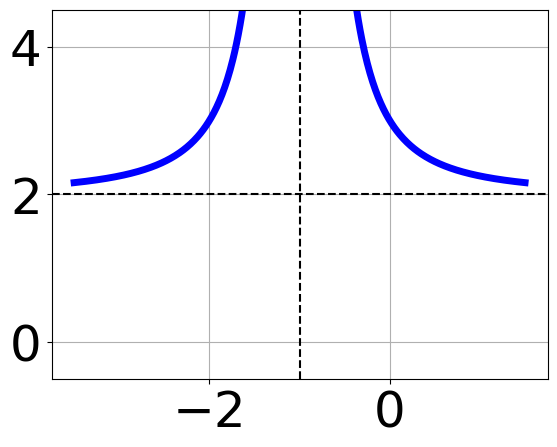
\includegraphics[width = 0.3\textwidth]{../Figures/rationalEquationToGraphCopyDA.png}\end{multicols}\item None of the above.
\end{enumerate} }
\litem{
Choose the equation of the function graphed below.
\begin{center}
    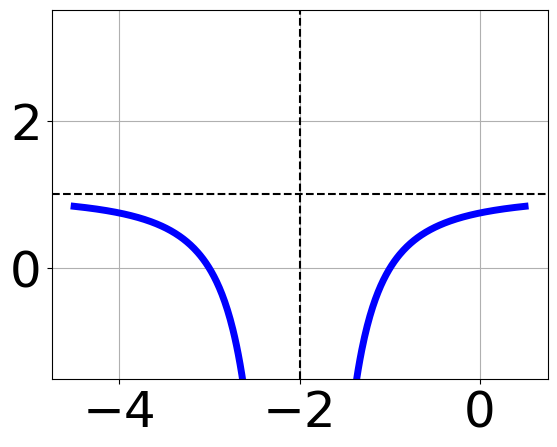
\includegraphics[width=0.5\textwidth]{../Figures/rationalGraphToEquationCopyA.png}
\end{center}
\begin{enumerate}[label=\Alph*.]
\item \( f(x) = \frac{1}{x - 2} + 3 \)
\item \( f(x) = \frac{-1}{x + 2} + 3 \)
\item \( f(x) = \frac{-1}{(x + 2)^2} + 3 \)
\item \( f(x) = \frac{1}{(x - 2)^2} + 3 \)
\item \( \text{None of the above} \)

\end{enumerate} }
\litem{
Choose the equation of the function graphed below.
\begin{center}
    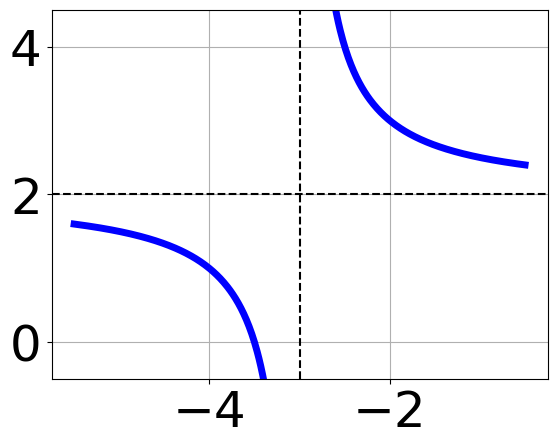
\includegraphics[width=0.5\textwidth]{../Figures/rationalGraphToEquationA.png}
\end{center}
\begin{enumerate}[label=\Alph*.]
\item \( f(x) = \frac{-1}{(x - 3)^2} + 2 \)
\item \( f(x) = \frac{1}{(x + 3)^2} + 2 \)
\item \( f(x) = \frac{1}{x + 3} + 2 \)
\item \( f(x) = \frac{-1}{x - 3} + 2 \)
\item \( \text{None of the above} \)

\end{enumerate} }
\litem{
Solve the rational equation below. Then, choose the interval(s) that the solution(s) belongs to.\[ \frac{54}{48x + 24} + 1 = \frac{54}{48x + 24} \]\begin{enumerate}[label=\Alph*.]
\item \( \text{All solutions lead to invalid or complex values in the equation.} \)
\item \( x \in [-0.5,1.5] \)
\item \( x \in [0.09,0.75] \)
\item \( x_1 \in [-0.59, 0.21] \text{ and } x_2 \in [0,1.1] \)
\item \( x_1 \in [-0.59, 0.21] \text{ and } x_2 \in [-1.2,-0.1] \)

\end{enumerate} }
\litem{
Choose the graph of the equation below.\[ f(x) = \frac{-1}{(x + 1)^2} + 1 \]\begin{enumerate}[label=\Alph*.]
\begin{multicols}{2}\item 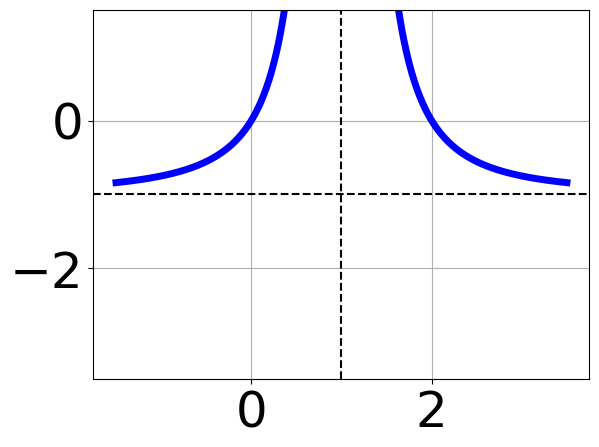
\includegraphics[width = 0.3\textwidth]{../Figures/rationalEquationToGraphAA.png}\item 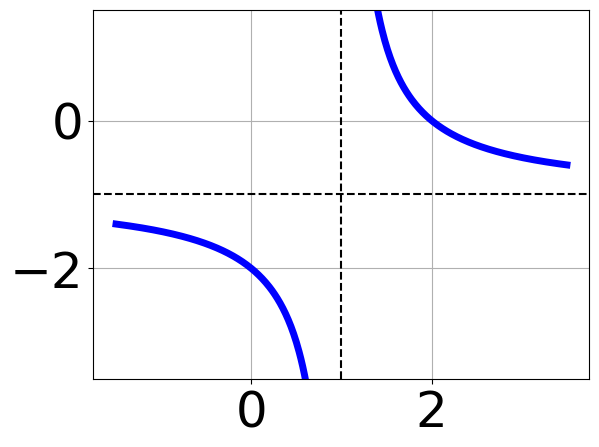
\includegraphics[width = 0.3\textwidth]{../Figures/rationalEquationToGraphBA.png}\item 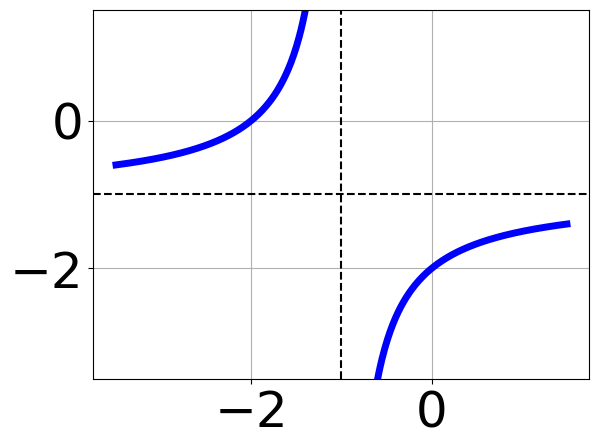
\includegraphics[width = 0.3\textwidth]{../Figures/rationalEquationToGraphCA.png}\item 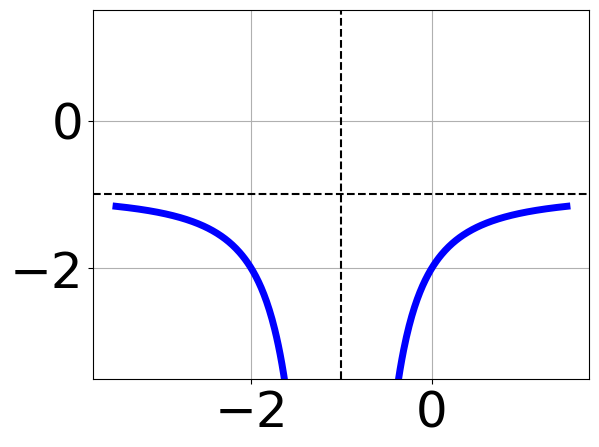
\includegraphics[width = 0.3\textwidth]{../Figures/rationalEquationToGraphDA.png}\end{multicols}\item None of the above.
\end{enumerate} }
\litem{
Solve the rational equation below. Then, choose the interval(s) that the solution(s) belongs to.\[ \frac{-2x}{3x -3} + \frac{-2x^{2}}{6x^{2} -24 x + 18} = \frac{-7}{2x -6} \]\begin{enumerate}[label=\Alph*.]
\item \( x \in [3.4,7.5] \)
\item \( \text{All solutions lead to invalid or complex values in the equation.} \)
\item \( x \in [0.8,3.4] \)
\item \( x_1 \in [-1, 0.9] \text{ and } x_2 \in [3.77,6.77] \)
\item \( x_1 \in [-1, 0.9] \text{ and } x_2 \in [-3,3] \)

\end{enumerate} }
\litem{
Determine the domain of the function below.\[ f(x) = \frac{6}{16x^{2} -12 x -18} \]\begin{enumerate}[label=\Alph*.]
\item \( \text{All Real numbers except } x = a, \text{ where } a \in [-13, -10] \)
\item \( \text{All Real numbers except } x = a, \text{ where } a \in [-0.75, 1.25] \)
\item \( \text{All Real numbers except } x = a \text{ and } x = b, \text{ where } a \in [-13, -10] \text{ and } b \in [23, 27] \)
\item \( \text{All Real numbers except } x = a \text{ and } x = b, \text{ where } a \in [-0.75, 1.25] \text{ and } b \in [1.5, 8.5] \)
\item \( \text{All Real numbers.} \)

\end{enumerate} }
\litem{
Solve the rational equation below. Then, choose the interval(s) that the solution(s) belongs to.\[ \frac{7x}{5x + 2} + \frac{-4x^{2}}{-10x^{2} +6 x + 4} = \frac{-3}{-2x + 2} \]\begin{enumerate}[label=\Alph*.]
\item \( x_1 \in [-1.45, 0.43] \text{ and } x_2 \in [-2.3,0.4] \)
\item \( x \in [1.24,2.03] \)
\item \( x_1 \in [-1.45, 0.43] \text{ and } x_2 \in [0.1,2] \)
\item \( x \in [0.9,1.67] \)
\item \( \text{All solutions lead to invalid or complex values in the equation.} \)

\end{enumerate} }
\litem{
Determine the domain of the function below.\[ f(x) = \frac{3}{15x^{2} -3 x -18} \]\begin{enumerate}[label=\Alph*.]
\item \( \text{All Real numbers except } x = a, \text{ where } a \in [-1, 0] \)
\item \( \text{All Real numbers except } x = a \text{ and } x = b, \text{ where } a \in [-11, -4] \text{ and } b \in [30, 34] \)
\item \( \text{All Real numbers.} \)
\item \( \text{All Real numbers except } x = a \text{ and } x = b, \text{ where } a \in [-1, 0] \text{ and } b \in [-0.8, 4.2] \)
\item \( \text{All Real numbers except } x = a, \text{ where } a \in [-11, -4] \)

\end{enumerate} }
\litem{
Solve the rational equation below. Then, choose the interval(s) that the solution(s) belongs to.\[ \frac{-3}{5x -4} + -9 = \frac{-3}{-25x + 20} \]\begin{enumerate}[label=\Alph*.]
\item \( x \in [0.72,1.72] \)
\item \( x_1 \in [0.72, 2.72] \text{ and } x_2 \in [0.79,0.96] \)
\item \( x_1 \in [-0.88, 0.12] \text{ and } x_2 \in [0.62,0.73] \)
\item \( \text{All solutions lead to invalid or complex values in the equation.} \)
\item \( x \in [-0.88,0.12] \)

\end{enumerate} }
\end{enumerate}

\end{document}